\documentclass{article}

\usepackage{geometry}
  \geometry{
    a4paper,
    right=25mm
  }

\usepackage{wrapfig}

\usepackage{graphicx}
\usepackage[latin1]{inputenc}
\usepackage[T1]{fontenc}
\usepackage[english]{babel}
\usepackage{listings}
\usepackage{xcolor}
\usepackage{eso-pic}
\usepackage{mathrsfs}
\usepackage{url}
\usepackage{amssymb}
\usepackage{amsmath}
\usepackage{multirow}
\usepackage{hyperref}
\usepackage{booktabs}
\usepackage{bbm}
\usepackage{cooltooltips}

\usepackage{colordef}
\usepackage{lvblisting}

\usepackage{algorithm}
\usepackage[noend]{algpseudocode}

\makeatletter
\def\BState{\State\hskip-\ALG@thistlm}
\makeatother

\DeclareMathOperator*{\argmin}{arg\,min}

\begin{document}
\section{Binary Response Models}
\subsection{Theory}

The outcome of interest in the Creditreform-dataset is of binary nature. Firms can either go bankrupt or not. This behavior is commonly modeled by Binary Response Models like the probit or the logit model. Binary response variables follow a Bernoulli probability function

\begin{equation}
f(y|x) = P(y=1|x)^y\left(1-P(y=1|x)\right)^{1-y},\qquad y\in \{0,1\},\; x\in \mathbb{R}^d, d \in \mathbb{N},
\end{equation}

where $P(y=1|x)$ stands for the conditional probability of observing $y=1$ given $x$. Both probit and logit models have in common that $P(y=1|x)$ is modeled by a monotonic transformation of a linear function

\begin{equation}
P(y=1|x) = G(x \prime \beta), \qquad \beta \in \mathbb{R}^d,
\end{equation}

where $x \prime \beta$ is the scalar product of $x$ and $\beta$. Additionally we require that $0 \leq G(x \prime \beta) \leq 1$, since it denotes a probability.

For the probit model $G$ will be the cumulative density function of the normal distribution

\begin{equation}
P(y=1|x) = G(x \prime \beta) = \Phi(x \prime \beta) = \int_{-\inf}^{x \prime \beta} \frac{1}{\sqrt{2\pi}}exp\left[-(\frac{t^2}{2})\right]dt.
\end{equation}

Here $\Phi(x \prime \beta)$ stands for the cumulative density function of the normal distribution.

For the logit model $G$ will be replaced by the cumulative density function of the logistic distribution $\Lambda(x \prime \beta)$:

\begin{equation}
P(y=1|x) = G(x \prime \beta) = \Lambda(x \prime \beta) = \frac{exp(x \prime \beta)}{1+exp(x \prime \beta)}
\end{equation}

The parameter vector $\beta$ is obtained by the Maximum-Likelihood method. Given independent and identically distributed samples, the Likelihood function can be written as

\begin{equation}
\begin{split}
L(\beta;y, x) &= \prod_{i=1}^{n} f(y_i | x_i)
              =\prod_{i=1}^{n} P(y_i=1|x_i)^y_i\left(1-P(y_i=1|x_i)\right)^{1-y_i} \\
            & =\prod_{i=1}^{n} G(x_i\prime \beta)^y_i\left(1-G(x_i\prime \beta)\right)^{1-y_i}
\end{split}
\end{equation}

where we just take the product over all individual Bernoulli-functions.

The log-Likelihood can thus be written as
\begin{equation}
\label{logL}
l = \log L(\beta;y x) = \sum_{i=1}^{n} y_i \log G(x_i\prime \beta) +(1-y_i) \log (1-G(x_i\prime \beta))
\end{equation}

The Maximum-Likelihood estimators $\beta_ML$ are calculated as

\begin{equation}
\beta_ML = argmax(l) \\
\end{equation}

and solve the first order conditions for a maximum.

\begin{equation}
\frac{\partial l}{\partial \beta} \stackrel{!}{=} 0
\end{equation}

In general, the resulting system of equations has no closed-form solution for $\beta_ML$ and numerical solutions are needed which can be obtained by iterative optimization techniques, one we will implement in the next section.

\subsection{Implementation}

The architecture of the \texttt{brm}-class follows the general structure outlined in the chapter before. First, it generates a log-Likelihood-function, which it then optimizes using a Gradient-Descent-Algorithm. After training the model it is possible for the user to very easily obtain predictions by invoking the \texttt{predict()}-function, which has been augmented with a method for the \texttt{brm}-class.

\subsubsection{Obtaining the Likelihood}

The first task is to define a function that accepts a distribution and yet undefined data as it's input and first extracts all suitable variables, then expresses the Likelihood-function from \ref{logL} and finally returns another function which depends only on the weights $\beta$. This task is performed by the \texttt{get\_likehood()}-function. We outline the function pass of \texttt{get\_likehood()} first in pseudo-code followed by a look on the implementation in the \texttt{R} language.

\begin{algorithm}
\caption{get\_likehood()}\label{getllog}
\begin{algorithmic}[1]
\Procedure{Set up auxiliary variables}{}
\State $\textit{grp} \gets \text{unique labels}$
\State $\textit{nums} \gets \text{extract numeric columns}$
\State $\textit{Xy\_mat} \gets \text{bind numeric variables as a matrix}$
\State $\textit{y\_pos} \gets \text{cache position of the outcome variable}$
\EndProcedure

\Procedure{Set up log-Likelihood}{}
\State $\textit{l} \gets 0$
\State \textbf{for}: $x_i, y_i \text{in data}:$
\State \qquad $\textbf{calculate}: j = y_i \log G(x_i\prime \beta) +
               (1-y_i) \log (1-G(x_i\prime \beta)$
\State \qquad $\textbf{update}: l \gets l + j$
\State $\textbf{return}: l(\beta)$
\EndProcedure
\end{algorithmic}
\end{algorithm}

The heavy lifting in this function is done by this \texttt{R}-snippet:
\lstinputlisting[language=R, firstline=15, lastline=25, firstnumber=15]{../BRM/logit.R}

The \texttt{for}-loop from the pseudo code is implemented as an \texttt{apply}-call to \texttt{Xy\_mat}, which in turn is a matrix of numeric columns. The \texttt{apply}-function initially selects each row in \texttt{Xy\_mat} and extracts the outcome-variable \texttt{Xy\_mat[y\_pos]} which corresponds to $y_i$ from \ref{logL}. It then computes the scalar product between the regressors of \texttt{Xy\_mat}'s row, which plays the role of $x_i \prime \beta$ in \ref{logL}. The scalar product is wrapped in \texttt{dist} which represents the cumulative distribution function $G(x\prime\beta)$ and is one of the arguments to \texttt{get\_loglikelihood()}.

\lstinputlisting[language=R, firstline=30, lastline=33, firstnumber=30]{../BRM/logit.R}

This way \texttt{dist} will point to the built-in functions for computing probabilities, depending if the user wishes to train a logit or a probit model. The arguments \texttt{lower.tail=TRUE} and \texttt{lower.tail=FALSE} stand for $G(x\prime \beta)$ and $G(x\prime \beta)= 1 - G(x\prime \beta))$ respectively. Finally the resulting vector is summed up and multiplied by $-1$. This is done because of the way we implemented the Gradient Descent algorithm. Currently \texttt{gradientDescentMinimizer()} can only find minima. However, Maximum-Likelihood estimation poses a maximization problem. Luckily, we can transform any maximization problem into a minimization problem by multiplying with minus one.

\subsubsection{Gradient Descent}

Since we now have a log-Likelihood function, the next step is to optimize it. To this effect we deploy a Gradient Descent algorithm. Theory tells us that in order to reach the minimum of a function $f(x)$ starting at a particular $x \in \mathbb{R}^d, d \in \mathbb{N}$ one needs to follow the negative gradient $\nabla f(x)$ of $f$ evaluated at $x$. This leads to the iterative rule we can exploit

\begin{equation}
\label{gradientDescent}
x_{t+1} = x_t - \eta \cdot \nabla f(x_t), \qquad t \in \mathbb{N}, \eta \in \mathbb{R}^+
\end{equation}

where $\eta$ is the learning rate. To this standard method of performing a Gradient Descent routine we will also make some minor modifications. First of all, we will approximate the gradients by taking finite differences, which is easier to implement albeit computationally inefficient. Finite differences are computed by

\begin{equation}
\label{finDiff}
\nabla f(x_t) \approx \frac{f(x_{t+1}) - f(x_t)}{\epsilon}, \qquad \epsilon > 0
\end{equation}

Secondly, we will before we initialize the algorithm, try a set of random points and chose the one that provides the lowest value of the objective function as a starting point for the Gradient Descent Routine. This also ensures to an extend that the algorithm, if it reaches convergence, finds the global minimum. The final modification will be to prune the gradients. When computing gradients using finite differences, it may happen that the gradient's values can become extremely high for large denominators and very small $\epsilon$. In fact, they can become high enough for \texttt{R} to treat them as \texttt{Inf} which results in the gradients being treated as \texttt{NaN} (not a number). To counteract that, we will limit the gradients to the interval $[-100, 100]$. 

\begin{algorithm}
\caption{gradientDescentMinimizer()}\label{GDM}
\begin{algorithmic}[1]
\Procedure{Set up auxiliary variables}{}
\State $\textit{learn\_rates}\gets \text{descending sequence from \texttt{learn} to 0}$
\State $\textit{a} \gets \text{matrix of 1000 randomly initialized points}$
\State $\textit{f\_a} \gets \text{vector of function values for each element of a}$
\State $\textbf{update:} a \gets \text{argmin(f\_a)}$
\State $\textit{gradient} \gets \textbf{compute gradient evaluated at a}$
\State $\textit{i} \gets 0$
\EndProcedure

\Procedure{Perform Gradient Descent}{}
\State $\textit{l} \gets 0$
\State \textbf{while}: $i \leq \textit{max\_iter} \text{ and any element of gradient} > 0:$
\State \qquad $\textbf{update}: a = a - \texttt{learn\_rates[i]} \cdot gradient$
\State \qquad $\textbf{calculate}: \textit{gradient} = \textbf{calculate gradient}$

\If {\text{i} = \text{max\_iter}} \textbf{raise} warning
\EndIf
\State $\textbf{return}: a$
\EndProcedure
\end{algorithmic}
\end{algorithm} 

The \texttt{gradientDescentMinimizer()}-function accepts following arguments:
\begin{enumerate}

\item \texttt{obj}: an objective function, that accepts exactly one argument called 'x'.
\item \texttt{n\_pars}: an integer specifying the dimensions of the objective.
\item \texttt{epsilon\_step}: a float defining the stepwidth used for computing the finite differences.
\item \texttt{max\_iter}: an integer for the maximum number of iteration before the algorithm aborts.
\item \texttt{precision}: a float defining the precision of the solution. All elements of the gradient have to be absolutely lower than \texttt{precision} for the algorithm to converge.
\item \texttt{learn}: a positive float representing the learning rate.
\item \texttt{verbose}: a boolean indicating if additional information during training is desired. The default is \texttt{FALSE}
\item \texttt{report\_freq}: If \texttt{verbose} is \texttt{TRUE}, define how often to print the logstring. The default is 10 which corresponds to a console output being printed every 10 steps.

\end{enumerate}

\lstinputlisting[language=R, firstline=143, lastline=148, firstnumber=143]{../BRM/utils.R}

We begin by filling the matrix \texttt{a} with 1000 \texttt{n\_pars}-dimensional points which we draw from the uniform distribution, making use of \texttt{R}'s built-in \texttt{runif}-function. We draw random numbers within the range of $[-100, 100]$ to cover a wide part of the objective function's domain.  

The workhorse in this routine is the \texttt{get\_gradient()}-function, which computes the finite differences. First we need to compute the values of the objective function at the current and next step (lines 146 and 147). Then we can apply the current and next step as inputs to the objective function and compute the difference $f(x_{t+1}) - f(x_t)$. The current step is provided as the \texttt{x} argument to the function call. The next steps need to be inferred by the function. If $f(x_t)$ is multidimensional we need to perform an $\epsilon$-step in each dimension of the vector, since we want to approximate the partial derivatives of $f(x)$ evaluated at $x_t$. I.e. first we want to increment just the first element of $x$ and store the result, then just the second element, and repeat the process until we reach the last element. If we stack these vectors, we get a matrix of one-directional $\epsilon$-steps that are essentially updates of the starting point $x_t$ with which it is easy to compute the gradients as their element-wise difference, normalized by \texttt{epsilon\_step}. The gradients are finally trimmed if necessary and returned.

\lstinputlisting[language=R, firstline=130, lastline=139, firstnumber=130]{../BRM/utils.R}

\begin{algorithm}
\caption{get\_gradient()}\label{getGrad}
\begin{algorithmic}[1]
\Procedure{Set up auxiliary variables}{}
\State $$\textit{init} \gets \begin{bmatrix}
x_1 & x_2 & \cdots\\
x_1 & x_2 & \cdots\\
x_1 & x_2 & \cdots\\
\vdots & \ddots & \cdots
\end{bmatrix} $$

\State $$\textit{steps} \gets 
\begin{bmatrix}
x_1 + \epsilon & x_2 & \cdots\\
x_1 & x_2 + \epsilon & \cdots\\
x_1 & x_2 & \cdots\\
\vdots & \ddots & \cdots
\end{bmatrix}$$

\State $\textit{f\_comp} \gets \textbf{apply row-wise:} \text{ objective function to } \textit{init}$
\State $\textit{f\_steps} \gets \textbf{apply row-wise:} \text{ objective function to } \textit{steps}$
\EndProcedure

\Procedure{Compute finite differences}{}
\State $$\textit{D} \gets \frac{f\_steps - f\_comp}{\epsilon}$$
\If{$any d \in D \notin [-100; 100]$} \textbf{replace} \text{d by 100 $\cdot$ sign(d)}
\EndIf
\EndProcedure
\end{algorithmic}
\end{algorithm}

\lstinputlisting[language=R, firstline=155, lastline=177, firstnumber=155]{../BRM/utils.R}

In each iteration the \texttt{while}-loop ensures that convergence has not been reached. This is implemented by a call to \texttt{any} wrapped around a vector of logical expressions. If any element of the gradient is still greater than the specified precision, the call to \texttt{any} will evaluate to \texttt{TRUE}. The second breaking criterion is a safeguard for the loop not to run infinite times. If the current iteration is larger than \texttt{max\_iter} the algorithm will break and the user will receive a warning (lines 175-176). If the user wishes to receive information about the status of the algorithm during runtime, the optional argument \texttt{verbose} can be set to \texttt{TRUE} which will print a logstring to the console in regular intervals (lines 156-161).

\subsubsection{Predictions}

In order to facilitate making predictions based on the \texttt{brm}-class we augmented the built-in function \texttt{predict()} with a method that works on our custom class in a predefined way.

\lstinputlisting[language=R, firstline=61, lastline=68, firstnumber=61]{../BRM/logit.R}

A call to \texttt{predict()} on a \texttt{brm}-model will add a column of ones to the provided \texttt{data} and multiply the matrix with the weights calculated during training of the model (line 62). Finally these scores of the index-function $X\beta$ will be applied to the correct distribution. The distribution is stored inside \texttt{model\$distribution} which points to \texttt{pnorm} in case of \texttt{brm}-model of \texttt{mode} "probit" and a pointer to \texttt{plogis} if the \texttt{mode} is equal to "logit". 

\section{Linear Discriminant Analysis}
\subsection{Theory}

Linear Discriminant Analysis (LDA) is a technique for dimensionality reduction that encorporates information on class-labels of the different observations. In contrast to  Principal Component Analysis, which is a unsupervised dimensionality reduction technique, it finds the rotation that ensures the highest separability between classes. It accomplishes this goal by trying to maximize between class variance while simultaneously minimizing within class variance.

\begin{equation}
max\ J_{b}(w) = w \prime S_{b} w, \qquad w \in \mathbb{R}^d, d \in \mathbb{N}
\end{equation}

\begin{equation}
min\ J_{w}(w) = w \prime S_{w} w
\end{equation}

This is done by maximizing the so called Raleigh coefficient
\begin{equation}
\label{LDA}
max J = \frac{J_b(w)}{J_w(w)} = \frac{w \prime S_{b} w}{w \prime S_{w} w}.
\end{equation}

The matrices for between and within class variance are defined as
\begin{equation}
S_b = \sum_{c=1}^{C}(\mu_c - \mu)(\mu_c - \mu)\prime
\end{equation}

\begin{equation}
\label{Sw}
S_w = \sum_{c=1}^{C}\sum_{i \in c}(x_i - \mu_c)(x_i - \mu_c)\prime
\end{equation} 

where $C$ is the number of classes, $\mu_c$ is the vector of sample means for each class respectively and $\mu$ is the vector of sample means for the full dataset. For identification purposes we can always chose weights $w$ such that $w\prime S_w w = 1$, since $J$ is constant with regards to rescalings. We can therefore replace $w$ by $\alpha w$ which will result in the constant $\alpha$ canceling out. This way the initial optimization problem can be formulated as

\begin{equation}
\argmin_{w} -\frac{1}{2} w\prime S_b w \quad s.t. \quad w \prime S_w w = 1
\end{equation}

with the lagrangian being

\begin{equation}
\mathcal{L} = -\frac{1}{2} w\prime S_b w + \frac{1}{2}\lambda\left(w\prime S_w w - 1\right).
\end{equation}

The halves are added for more convenient matrix derivatives. The Karush-Kuhn-Tucker conditions imply that the solution to this maximization problem and subsequently the vector of weights we want to find needs to fulfill

\begin{equation}
\label{LDAsolution}
S_b w = \lambda S_w w.
\end{equation}

This is a generalized eigenvalue problem for which there exists a convenient \texttt{R}-solution in the form of the \texttt{geigen}-package.

\subsection{Implementation}

The result from \ref{LDAsolution}, which is essentially the rotation of the underlying data's column space that ensures the highest separability, is implemented in the \texttt{lda}-class for the two-class case. The \texttt{lda()} function accepts two arguments:

\begin{enumerate}
\item \texttt{data}: a \texttt{data.frame} containing at least one column of factors indicating the class label.
\item \texttt{by}: a \texttt{character}-string equal to the column's name containing the class labels. Note that all other non-numerical columns will be ignored by the function, since LDA is only meaningful for continuous variables.
\end{enumerate} 

The function in a first step extracts the useable columns and the number of classes provided in \texttt{data}. It then performs a quick check if the prerequisites are met and then continues with the calculation of the class-means $\mu_1$ and $mu_2$, the overall mean $\mu$, as well as the scatter-matrices $S_b$ and $S_w$. With these we can solve the generalized eigenvalue problem from \ref{LDAsolution}.

\begin{algorithm}
\caption{\texttt{lda()}} \label{lda-function}
\begin{algorithmic}[1]
\Procedure{Set up Auxiliary Variables}{}
\State $\textit{num} \gets \textbf{extract numeric columns}$
\State $\textit{classes} \gets \textbf{extract class labels}$
\State $\textit{mu} \gets \textbf{calculate class means}$
\State $\textit{x\_bar} \gets \textbf{calculate overall means}$
\State $\textit{S} \gets \textbf{calculate variance per group}$
\State $\textit{S\_b1 \& S\_b2} \gets \textbf{get summands for between class scatter matrix}$
\EndProcedure

\Procedure{Calculate Scatter Matrices}{}
\State $\textit{S\_b} \gets \texttt{S\_b1 + S\_b2}$
\State $\textit{S\_w} \gets \texttt{S[[[1]] + S[[2]]}$
\EndProcedure

\Procedure{Solve Generalized Eigenvalue Problem}{}
\State $\textit{V} \gets \textbf{calculate Eigenvectors and Eigenvalues}$
\State $\textit{v} \gets \textbf{extract 2 Eigenvectors associated to largest Eigenvalues}$
\State $\textit{lda1 \& lda2} \gets \textbf{calculate first two LDA-Components}$
\State $\textit{inertia} \gets \textbf{calculate percentage of explained variance}$
\State $\textbf{return: } \texttt{lda1, lda2, classes, mu, v, inertia}$
\EndProcedure

\end{algorithmic}
\end{algorithm}

The first task of the \texttt{lda()}-function is to determine, if the prerequisites for further computation are met. To this avail it first asserts that the user provided a dataframe that contains at least one numeric column and a column that contains exactly two distinct class labels (lines 11-17). In a second step it calculates all required variables such as the class means $\mu_1$ and $\mu_2$, the overall mean $\mu$ and the covariance matrices for each group (lines 18-19). The class specific metrics are computed by calls to custom made functions defined in the \texttt{utils.R}-file of the \texttt{LDA}-directory. Essentially these functions are wrappers for subsetting a provided dataframe by a provided key, here this is the class-label, and and an \texttt{apply} call looping over the respective subset's columns. The \texttt{get\_class\_means()} calculates the mean inside the \texttt{apply}-function whereas \texttt{get\_class\_cov()} uses a call to the built-in \texttt{cov}-function. However note that \texttt{cov} calculates 

$$\hat{cov}(X) = \frac{1}{N-1} \sum_{i = 1}^{N}(x_i - \bar{x})(x_i - \bar{x})\prime.$$

Unfortunately this is not exactly what we want for the scatter matrix defined in \ref{Sw}. We need to multiply the resulting list of covariance matrices elementwise by the number of observations in each class minus one. We correct this before calculating the within class scatter matrix on line 31. 

\lstinputlisting[language=R, firstline=6, lastline=31, firstnumber=6]{../LDA/lda.R}

With the \texttt{matrix}-object \texttt{S\_w} storing the within-scatter-matrix $S_w$ and \texttt{S\_b} storing $S_b$ we can continue by solving the generalized Eigenvalue problem posed in \ref{LDAsolution}. This is done by the \texttt{geigen()} function from the \texttt{geigen} package.

\lstinputlisting[language=R, firstline=36, lastline=43, firstnumber=36]{../LDA/lda.R}

We extract the eigenvectors and eigenvalues from \texttt{V} (line 36) in form of a list. However, caution is required because the eigenvectors are not ordered, which is different to the implementation of eigenvalues in the \texttt{base}-function \texttt{eigen()}. Therefore we rearrange the eigenvectors according to their absolute eigenvalues (line 39). We extract only the first two eigenvectors, because we require the most informative rotations in order to produce two-dimensional plots. Additionally we compute the percentage of explained variance as 

\begin{equation}
intertia_i = \frac{\lambda_i^2}{\sum_{j=1}^{d}\lambda_{j}^{2}}.
\end{equation}

The rotations \texttt{lda1} and \texttt{lda2} are computed by an \texttt{apply}-call (lines 45-46) to an anonymous function which emulates a scalar product by multiplying the two vectors \texttt{v[, i]}, which is the $i$-th eigenvector $i \in \{1, 2\}$, with each observation in the provided dataset. Computationally this is equivalent to the matrix multiplication $Xv_i$, where $X$ is the data matrix and $v_i$ is the eigenvector.

Finally we gather the results into a \texttt{list} and sets it's class to \texttt{flda}. This allows us to augment pre-existing functions with a custom method for predicting and plotting for future objects of the\texttt{flda}-class in an object-oriented fashion.

\subsubsection{Plotting}

With a trained model of the \texttt{flda}-class it may be of interest to plot the rotations in order to get a visualisable idea of the separability of the two classes. To make this as easy as possible for the end-user we implemented a \texttt{plot} method for each instance of a \texttt{flda}-class. This means that a user can simply store a call to the \texttt{lda}-function inside a variable, called \texttt{model} for example. To plot the rotations one can simply invoke \texttt{plot} on \texttt{model} as easy as with any other model class by typing \texttt{plot(model)}.

This is done by augmenting \texttt{R}'s \texttt{plot}-function using the \texttt{plot.\_\_className\_\_} syntax. Here we replace \texttt{\_\_className\_\_} by \texttt{flda}

\lstinputlisting[language=R, firstline=61, lastline=69, firstnumber=61]{../LDA/lda.R}

We overwrite the behavior of \texttt{plot} in order to accomodate \texttt{flda}-objects. Here we pass the model's precomputed rotations to the \texttt{ggplot2} function. The \texttt{ggplot2::\_\_function\_\_} makes it explicit that we want the \texttt{\_\_function\_\_} from the \texttt{ggplot2} package. Another benefit of this syntax is that this way we do not implicitly change a users namespace, which may potentially hide some functions by overwriting them with \texttt{ggplot2} routines and therefore may result in unexpected behavior.

Looking at the creditreform dataset we can apply our custom routines by creating a train-set first and then visualizing the results. This reveals already why LDA's predictive results are of poor quality. The feature space spanned by the financial ratios is simply not linearly separable.


\lstinputlisting[language=R, firstline=19, lastline=21, firstnumber=19]{../LDA/creditLDA.R}

\begin{figure}
\caption{Using Linear Discriminant Analysis on the Creditreform Database}
\centering
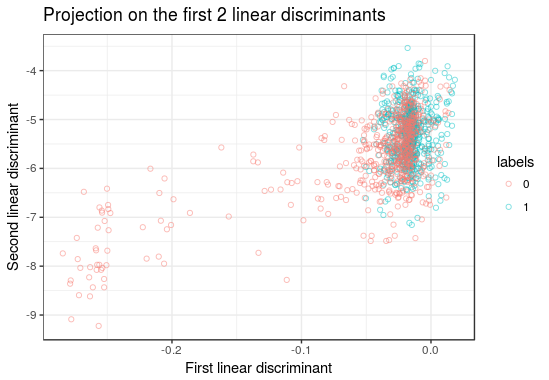
\includegraphics{../LDA/creditLDA.png}
\end{figure}

\subsubsection{Predictions}

To make predicting with the \texttt{flda}-class as easy as plotting we augment the standard \texttt{predict} function in a similar fashion. We expect the user to have already trained an \texttt{flda}-model to which she or he wishes to apply new data and obtain predictions on the class labels. 

\lstinputlisting[language=R, firstline=71, lastline=88, firstnumber=71]{../LDA/lda.R}

The provided new data should have a similar structure to the training data. This means that especially the order of the columns should be the same. We check for obviously non-conforming data in line 77 but we do not perform explicit tests on the order of columns. If the data has the required shape we calculate the discriminant function for each observation, which is the scalar product of the observation's data vector and the first eigenvector from the trained model. We then proceed calculating a threshold $c$ for being able to discriminate between the two groups by following the rule

\begin{equation}
c = \frac{1}{2} v \prime \left(\mu_1 + \mu_2\right) 
\end{equation}

predictions are made according to the threshold, if the value of the discriminant function is smaller than the threshold we assign the label of the first class and the second class otherwise. 
 
\section{Appendix}

\subsection{Unit Tests}
\subsubsection{LDA}

\begin{wrapfigure}{r}{0.3\textwidth}
\label{iris}
\begin{center}
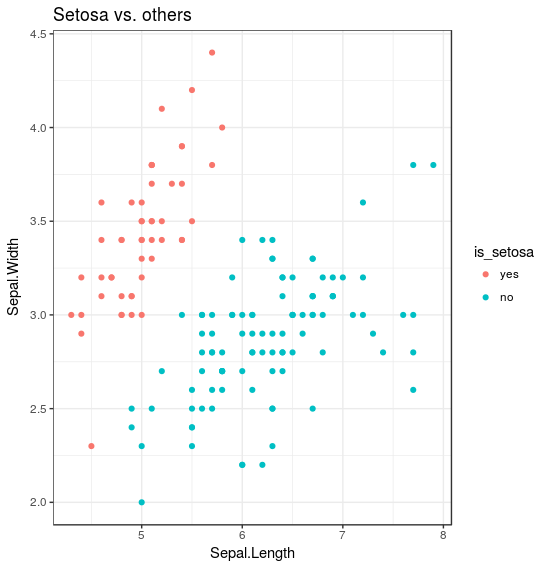
\includegraphics[scale=0.3, trim={10mm 20mm 30mm 30mm}]{../LDA/iris.png}
\end{center}
\caption{The Setosa-Species is already almost separable, even in the normal space.}
\end{wrapfigure}


In order to test the \texttt{lda}-function we take a dataset from which we know that it is linearly separable already and see if we can reproduce the results. Since Linear Discriminant Analysis was first proposed by Sir Ronald A. Fisher it is only fitting that we test it on his famous \texttt{iris} dataset. The \texttt{iris} dataset contains measurements for the sepal and petal length and width of three different species of iris flowers. We know that the sepal length and the petal length are sufficient variables to create a obviously visible separation line in figure \ref{iris} which discriminates the Setosa-species almost perfectly from the rest. 

Should the \texttt{lda}-function work as intended we would expect this result only to become better, i.e. the points being perfectly separable.

The \texttt{iris}

\subsubsection{Binary Response Models}
\subsubsection{Evaluation}

\begin{thebibliography}{9}
\bibitem{winkel09}
  Winkelmann, R., Boes, S. (2009): \textit{"Analysis of Microdata"}, 2nd edition.
\end{thebibliography}
\end{document}